\documentclass[10pt]{article}

\usepackage{answers,setspace,graphicx,multicol,enumitem,textcomp}
\usepackage{mathrsfs,svg,adjustbox}
\usepackage[margin=1in]{geometry} 
\usepackage{totcount,xcolor,layout,latexsym,times,subfigure}
\usepackage{epsf,prooftrees,natded}
\input{epsf}
\usepackage[normalem]{ulem}
\usepackage{amsmath,amsthm,amssymb,xspace,multirow,graphicx,turnstile, float}
\usepackage[titlenotnumbered,noend,noline]{algorithm2e}
 
\newcommand{\N}{\mathbb{N}}
\newcommand{\Z}{\mathbb{Z}}
\newcommand{\C}{\mathbb{C}}
\newcommand{\R}{\mathbb{R}}
\newcommand{\Q}{\mathbb{Q}}
\newcommand{\Jas}{Ja\'skowski }
\newcommand{\JasA}{Ja\'skowski}
\newcommand{\KM}{Kalish-Montague }
\newcommand{\KMa}{Kalish-Montague}

\DeclareMathOperator{\sech}{sech}
\DeclareMathOperator{\csch}{csch}
 
\newenvironment{theorem}[2][Theorem]{\begin{trivlist}
\item[\hskip \labelsep {\bfseries #1}\hskip \labelsep {\bfseries #2.}]}{\end{trivlist}}
\newenvironment{definition}[2][Definition]{\begin{trivlist}
\item[\hskip \labelsep {\bfseries #1}\hskip \labelsep {\bfseries #2.}]}{\end{trivlist}}
\newenvironment{proposition}[2][Proposition]{\begin{trivlist}
\item[\hskip \labelsep {\bfseries #1}\hskip \labelsep {\bfseries #2.}]}{\end{trivlist}}
\newenvironment{lemma}[2][Lemma]{\begin{trivlist}
\item[\hskip \labelsep {\bfseries #1}\hskip \labelsep {\bfseries #2.}]}{\end{trivlist}}
\newenvironment{exercise}[2][Exercise]{\begin{trivlist}
\item[\hskip \labelsep {\bfseries #1}\hskip \labelsep {\bfseries #2.}]}{\end{trivlist}}
\newenvironment{solution}[2][Solution]{ \begin{trivlist}
\item[\hskip \labelsep {\bfseries #1}]}{\end{trivlist}}
\newenvironment{problem}[2][Problem]{\begin{trivlist}
\item[\hskip \labelsep {\bfseries #1}\hskip \labelsep {\bfseries #2.}]}{\end{trivlist}}
\newenvironment{question}[2][Question]{\begin{trivlist}
\item[\hskip \labelsep {\bfseries #1}\hskip \labelsep {\bfseries #2.}]}{\end{trivlist}}
\newenvironment{corollary}[2][Corollary]{\begin{trivlist}
\item[\hskip \labelsep {\bfseries #1}\hskip \labelsep {\bfseries #2.}]}{\end{trivlist}}
 
\begin{document}
 
% --------------------------------------------------------------
%                         Start here
% --------------------------------------------------------------
 
\title{Assignment 3}%replace with the appropriate homework number
\author{Aditya Arora\\ %replace with your name
Winter 2018\\$Quidquid\ Latine\ dictum\ sit,\ altum\ viditur$} %if necessary, replace with your course title
\maketitle

%Below is an example of the problem environment
\begin{problem}{1}
If you roll a fair dice $n$ times:
\begin{enumerate}
    \parskip=0in
    \parsep=0in
    \itemsep=0.1in
    \item How many times will the sequence 1,2,3,4,5,6 occur?  What is the probability of this occurring?
    \item How many times will the sum of the number of 1's and 2's equal the sum of the number of 3's, 4's, 5's and 6's?  What is the probability of this occurring?
    \item How many times will the sum of the number of 1's and 2's equal the sum of the number of 3's and 4's and equal the sum of the number of 5's and 6's?  What is the probability of this occurring?
    \item How many times will you roll a 1 twice in succession?  For the purpose of this calculation, the sequence ...11.... counts as once, but so does ...111....  The sequence ...1111... counts as twice.  What is the probability of this occurring?
    \item How many times will you roll a 1 $k$-times in succession?  As with the previous case, when a 1 is counted as part of a $k$-sequence, it is not counted as part of a subsequent $k$-sequence.  What is the probability of this occurring?
    \item You have a communications system that transmits bundles of data from a source to a destination.  Most bundles are received correctly. However, there is a random chance of the data in a bundle being in error.  Roughly every $E^{th}$ bundle is in error.  If you transmit $n$ bundles, what is the probability of two bundles in sequence being in error?  what is the probability of $k$ bundles in sequence being in error?
\end{enumerate}

You may wish to modify your Lab3 program {\tt dice} to give you a
sense of whether or not your answers look correct.
\end{problem}

%Below is the solution environment
\begin{solution}{1}
\item[]
\begin{enumerate}
    \parskip=0in
    \parsep=0in
    \itemsep=0.1in
\item
\end{enumerate}
\end{solution}



\vskip 0.5in
\newpage
\begin{problem}{2}
Prove (using induction) the binomial theorem:
\[
(x+a)^n = \sum_{r=0}^n{^{n}C_{r}}\ x^{n-r}a^r
\]
\end{problem}
\begin{solution}{2}
\item[] 
\[
P(y) = (x+a)^y = \sum_{r=0}^y{^{y}C_{r}}\ x^{y-r}a^r\]
We will first see if $P(1)$ is true
\[
P(1) = (x+a)^1 = x^1 + a^1 = \sum_{r=0}^1{^{1}C_{r}}\ x^{1-r}a^r
\]
Thus we can see that $P(1)$ is True

Let us assume that $P(m)$ is true. This means that 
\[P(m)  = (x+a)^m = \sum_{r=0}^m{^{m}C_{r}}\ x^{m-r}a^r
\]
Now using $P(m)$ we will try to prove $P(m+1)$\\
We know $P(m) * (x+a) = P(m+1)$\\
Thus: \[P(m+1) = {\sum_{r=0}^m{^{m}C_{r}}\ x^{m-r}a^r } * (x+a) \]
\[\Rightarrow P(m+1) = {\sum_{r=0}^m{^{m}C_{r}}\ x^{m+1-r}a^r } + {\sum_{r=0}^m{^{m}C_{r}}\ x^{m-r}a^{r+1} } \]
\[\Rightarrow P(m+1) = {\sum_{r=0}^m{^{m}C_{r}}\ x^{m+1-r}a^r } + {\sum_{r=1}^m{^{m}C_{r-1}}\ x^{m+1-r}a^{r} } \]
\[\Rightarrow P(m+1) = {{^{m}C_{0}}\ x^{m+1}a^0}+  {\sum_{r=1}^m{^{m}C_{r}}\ x^{m+1-r}a^r } + {\sum_{r=1}^m{^{m}C_{r-1}}\ x^{m+1-r}a^{r} }\] 
$$[Re-indexing\ the\ sum]$$
\[\Rightarrow P(m+1) = {{^{m+1}C_{0}}\ x^{m+1}a^0}+  {\sum_{r=1}^m({^{m}C_{r}}\ x^{m+1-r}a^r + {^{m}C_{r-1}}\ x^{m+1-r}a^{r}}) \]
$$[{^{m}C_{0}} = {^{m+1}C_{0}}]$$
\[\Rightarrow P(m+1) = {{^{m+1}C_{0}}\ x^{m+1}a^0}+  {\sum_{r=1}^m({^{m}C_{r}}+ {^{m}C_{r-1}})\ x^{m+1-r}a^r} \]
\[\Rightarrow P(m+1) = {{^{m+1}C_{0}}\ x^{m+1}a^0}+  {\sum_{r=1}^m{^{m+1}C_{r}}\ x^{m+1-r}a^r} \]
$$[{^{m}C_{r-1}} + {^{m}C_{r}} = {^{m+1}C_{r}}]$$
\[\Rightarrow P(m+1) = {\sum_{r=0}^m{^{m+1}C_{r}}\ x^{m+1-r}a^r} \]
$$[Re-indexing\ the\ sum]$$\\

Thus we have shown that if $P(m)$ is true we can show that $P(m+1)$ is True. \\

Thus we can say that using the principal of mathematical induction that $
(x+a)^n = \sum_{r=0}^n{^{n}C_{r}}\ x^{n-r}a^r
$ is True


\end{solution}


\pagebreak
\pagebreak
\newpage
\clearpage
\begin{problem}{3}
Is there
\begin{enumerate}
    \parskip=0in
    \parsep=0in
    \itemsep=0.1in
    \item a graph with 5 vertices and 3 edges?
    \item a graph with 5 odd-degree vertices with 3 edges?
    \item a connected graph with 5 vertices and 3 edges?
    \item a directed graph with 5 vertices and 3 edges?
    \item a disconnected graph (a graph that is not connected) with 5
vertices and 7 edges?
    \item a disconnected, directed graph with 5 vertices and 7 edges?
    \item a graph with 3 vertices and 5 edges?
    \item a directed graph with 3 vertices and 5 edges?
\end{enumerate}

In each case, if there exists such a graph, illustrate it; if not, explain (precisely) why not.
\end{problem}
\begin{solution}{3}
\item[]
\begin{enumerate}
\item Yes there is a graph with 5 vertices and 3 edges \\ 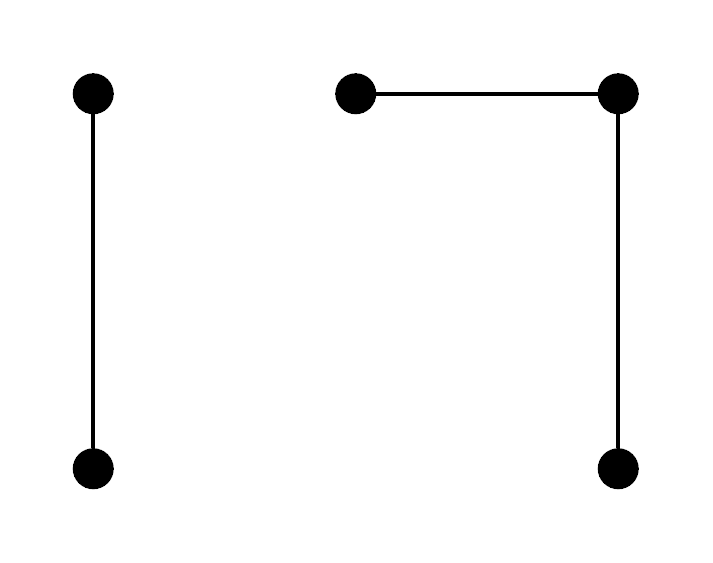
\includegraphics[width=4cm]{graph1}
\item No there does not exist a graph with 5 odd-degree vertices because the sum of all degrees is always even (because the sum of all the degrees is equal to twice the number of edges), but with 5 odd-degree vertices the sum would be odd.
\item No there does not exist a connected graph with 5 vertices and 3 edges because every connected graph with v vertices needs to have at least v - 1 edges
\item 
\item No there does not exist a dis-connected graph with 5 vertices and 7 edges. If we try to use 4 connected vertices and 1 disconnected vertex, we only end up with 6 edges\\
\begin{figure}[H]
    \centering
    \caption{Graph with 4 connected vertices}
    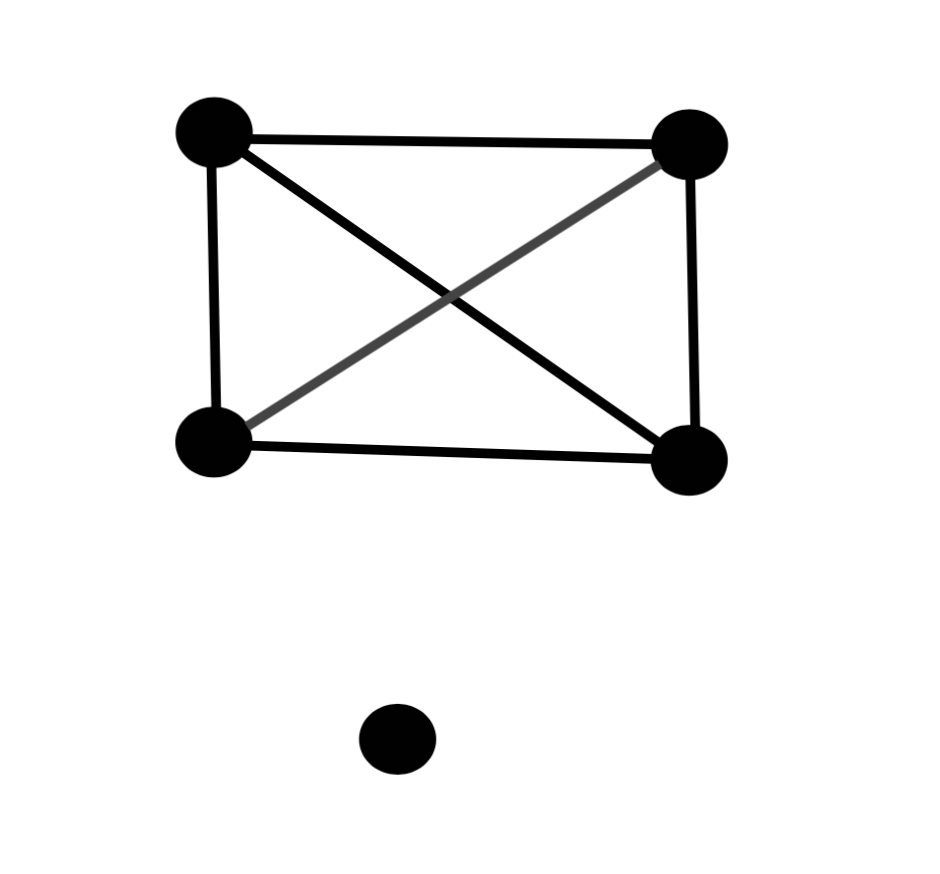
\includegraphics[width=4cm]{graph2}
\end{figure}
\pagebreak
If we use 2 connected components, one with 3 connected vertices and one with 2 connected vertices. We still end up with 4 edges\\
\begin{figure}[H]
    \centering
    \caption{Graph with 2 connected components}
    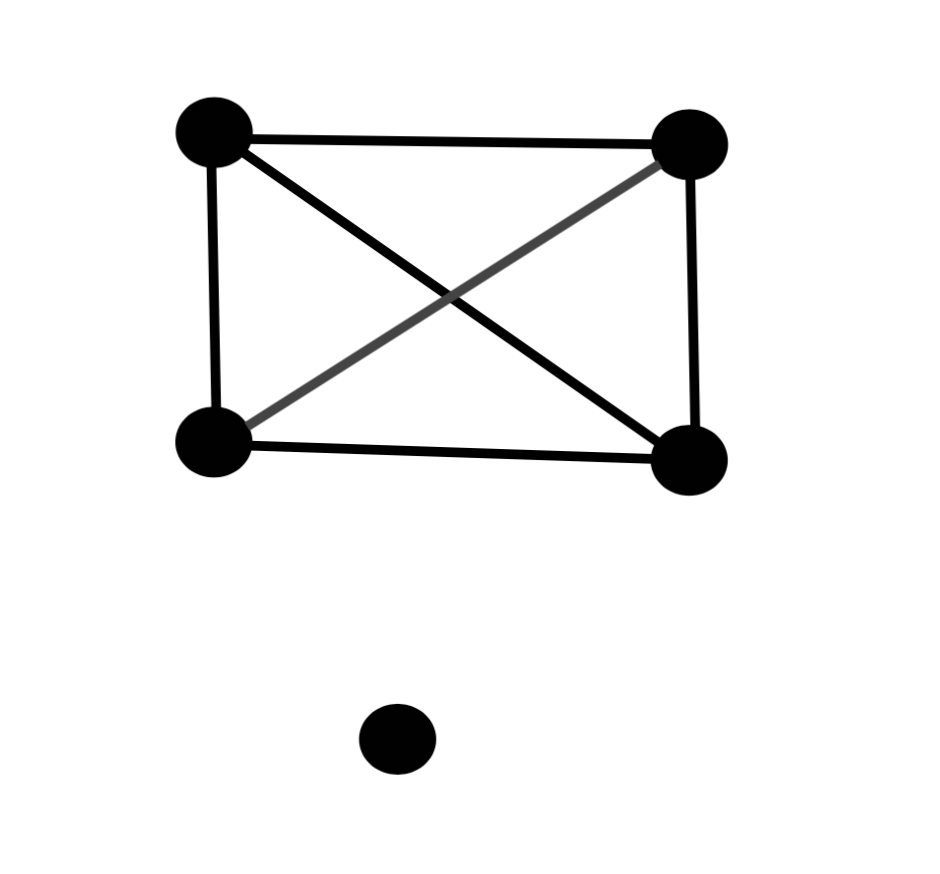
\includegraphics[width=4cm]{graph2}
\end{figure}

If we move to 3 connected components we get only 2 edges
\begin{figure}[H]
    \centering
    \caption{Graph with 3 connected components}
    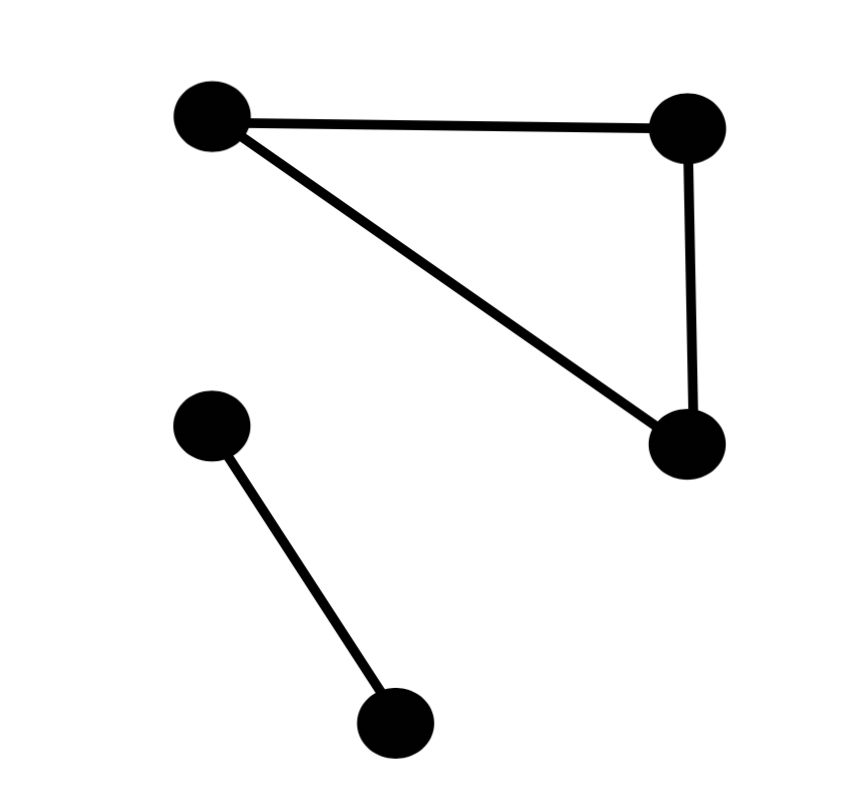
\includegraphics[width=4cm]{graph3}
\end{figure}
\item Shown below is a graph that is disconnected, directed graph and has 5 vertices and 7 edges
\begin{figure}[!h]
    \centering
    \caption{a disconnected, directed graph with 5 vertices and 7 edges}
    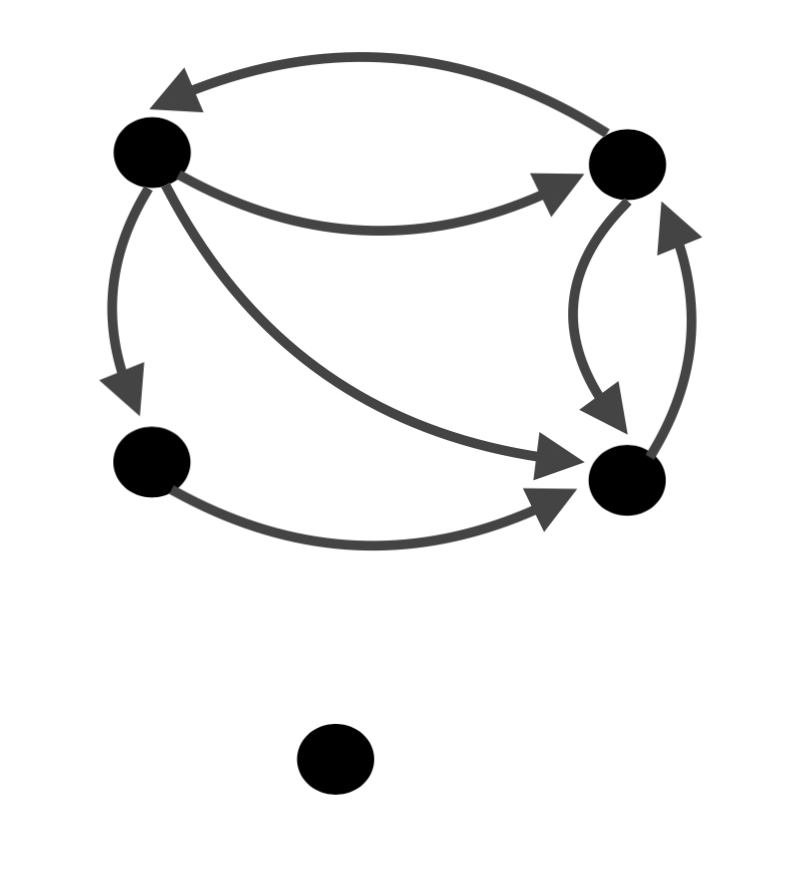
\includegraphics[width=4cm]{graph5}
\end{figure}
\item No there does not exist a graph with 3 vertices and 5 edges. The maximum number of edges possible are $^3C_2 = 3$
\newpage 
\item Shown below is a graph that is a directed graph with 3 vertices and 5 edges
\begin{figure}[!h]
    \centering
    \caption{a directed graph with 3 vertices and 5 edges}
    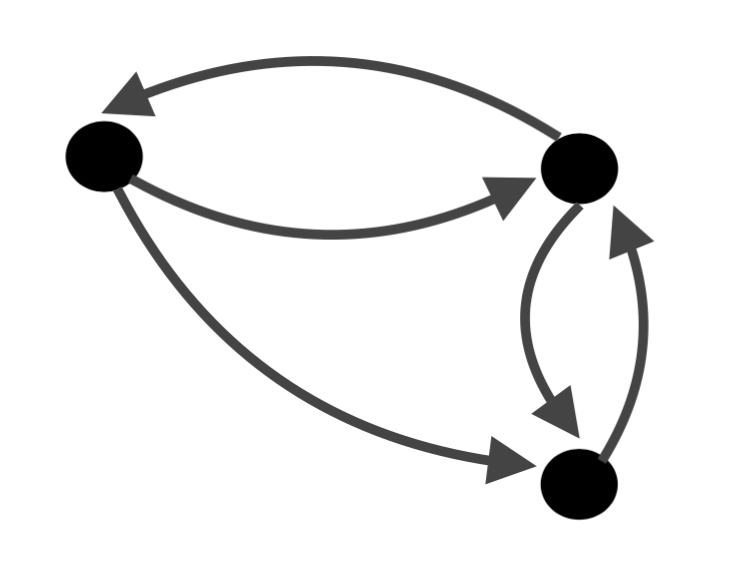
\includegraphics[width=4cm]{graph6}
\end{figure}

\end{enumerate}
\end{solution}

\vskip 0.5in
\newpage
\pagebreak
\pagebreak\newpage

\begin{problem}{4} Given the following graph:

\begin{center}
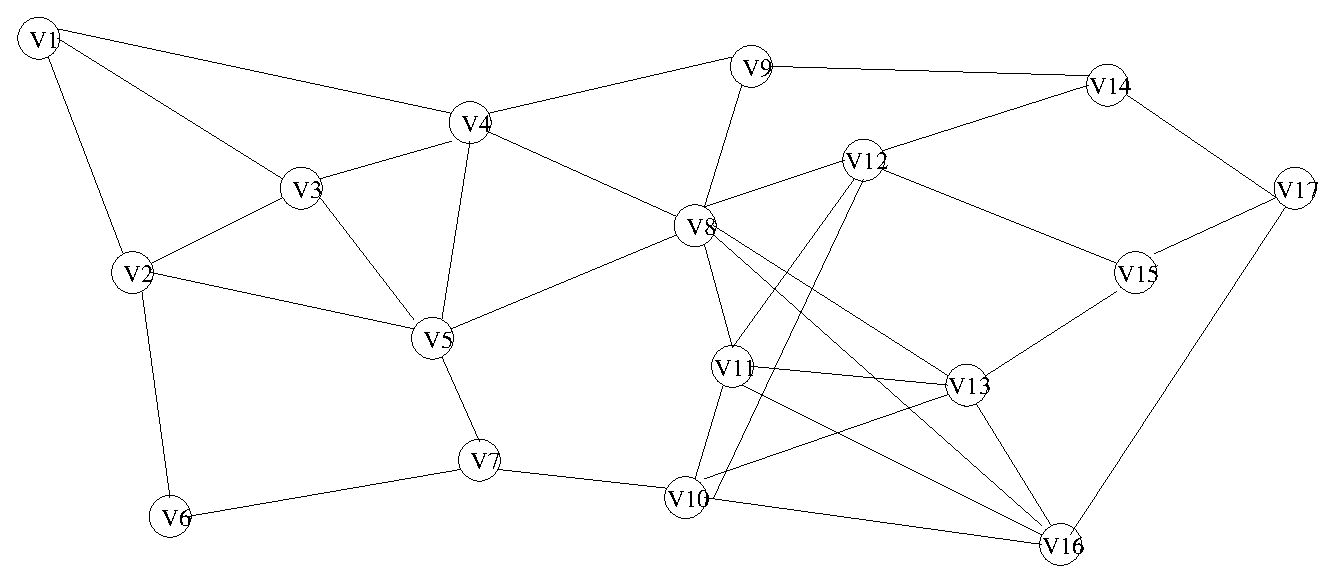
\includegraphics[scale=0.7]{graph.eps}
\end{center}
\begin{enumerate}
    \parskip=0in
    \parsep=0in
    \itemsep=0.1in
    \item Is this graph connected?
    \item Is this graph complete?  Why/Why not?
    \item What is the minimum degree of the graph?
    \item What is the maximum degree of the graph?
    \item What is the largest clique in the graph?
    \item Is the graph planar? Why/Why not?
    \item What is the shortest path from V1 to V17? How long is it?
    \item What is the longest path from V1 to V17?  How long is it?
\end{enumerate}
\end{problem}
\begin{solution}{4}
\item[]
\begin{enumerate}
    \parskip=0in
    \parsep=0in
    \itemsep=0.1in
    \item Yes the graph is connected since every pair of vertices are connected
    \item No the graph is not complete because every two vertices are not connected. Eg: Vertices $V_3$ and $V_15$ are not directly connected
    \item The minimum degree of the graph is 2
    \item The maximum degree of the graph is 7
    \item
    \item n = 17, m = 35 
    \item The shortest path is of length 4 and is $V1 \rightarrow V4 \rightarrow V9 \rightarrow V{14}
    \rightarrow V{17}$
    \item The longest path has 16 edges i.e. length 16 and is $V1\rightarrow V2\rightarrow V6\rightarrow V7\rightarrow V5\rightarrow V3\rightarrow V4\rightarrow V8\rightarrow V9\rightarrow V14\rightarrow V12\rightarrow V10\rightarrow V11\rightarrow V16\rightarrow V13\rightarrow V15\rightarrow V17$
\end{enumerate}
\end{solution}

\vskip 0.5in
\pagebreak

% \vskip 0.5in

% \begin{problem}{12}
% \item[]
% \begin{enumerate}[label=\alph*)]
% \end{enumerate}
% \end{problem}
% \begin{solution}{7}
% \item[]
% \begin{enumerate}[label=\alph*)]
% \end{enumerate}
% \end{solution}




\end{document}
